\documentclass{CUCProposal}

% 使用该宏包可以为参考文献、图表、公式添加超链接。但是可能会影响观感,可根据需要自行选择是否使用。
% 默认样式:使用方框标识超链接,很多期刊论文中有用
\usepackage[]{hyperref}
% 简化样式:不用方框,看起来会简洁一点,有各种颜色标识不同的类别
% \usepackage[colorlinks,linkcolor=red,anchorcolor=blue,citecolor=green]{hyperref}
% 保险样式:都是黑色的超链接,可以点击
% \usepackage[colorlinks,linkcolor=black,anchorcolor=black,citecolor=black,urlcolor=black]{hyperref}

% 中文占位符,可删除
\usepackage{zhlipsum}

% 参考文献文件位置,没有参考文献的话忽略即可
\addbibresource{ref.bib}

% 个人信息设置
\setup{
  % 姓名
  Name = 王小帅,
  % 学号
  StudentID = 201111111111,
  % 指导老师
  Advisor = 王大帅,
  % 专业
  Subject = 广播电视工程,
  % 毕设题目
  Title = 基于BSC模板的表格类文件 \LaTeX 实现方法研究,
  % 导师pdf电子签名
  AdvisorSign = {
\includegraphics[width=3cm]{Albus}},
  % 日期
  Date = 2022年12月25日
}

% 正文
\begin{document}
\makeKTtable{
% =====================开题报告内容=====================
\section{第一部分内容}
\zhlipsum[1]
\subsection{其中的内容}

适当引用文献\cite{rengongzhinengjianshi},适当引用文献\cite{zhongguozhexueshi},,适当引用文献\cite{jiqixuexi},适当引用文献\cite{vaswani_attention_2017},序号与本报告最后的参考文献一致。

\zhlipsum[1]

% 插入图片
\noindent
\begin{center}
  \begin{minipage}{0.8\linewidth}
  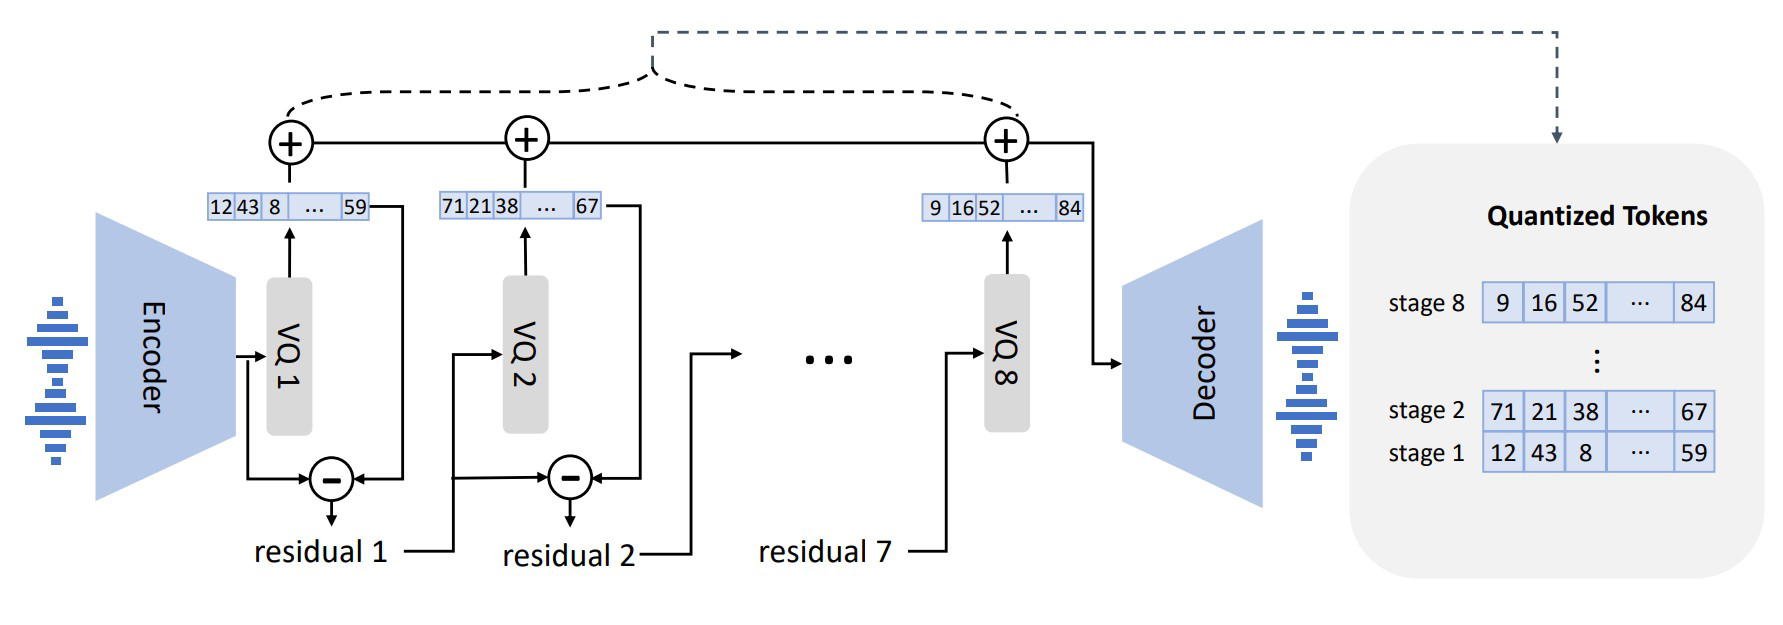
\includegraphics[width=\textwidth]{pic/VALL-E编码模型}
  \captionof{figure}{VALL-E编码模型\label{fig:examplefig}}
  \end{minipage}
\end{center}

% 插入表格
\begin{center}
  \singlespacing
  \begin{minipage}{.5\linewidth}
    \begin{center}
      \captionof{table}{An example table\label{tab:exampletable}}
      \begin{tblr}{colspec={ll},hline{1,2,Z}}
        Name&Schoolo\\
        Harry Potter&Gryffindor\\
        Draco Malfoy&Slytherin\\
      \end{tblr}
    \end{center}
  \end{minipage}      
\end{center}

注意!文中出现的图片、表格、公式等,都需要在文中进行引用!如图\ref{fig:examplefig}、表\ref{tab:exampletable}、公式\ref{eq:exampleeq}等。

% 公式
\begin{equation}
  E = mc^2 
  \label{eq:exampleeq}
\end{equation}

% 文字
\zhlipsum[1]
\zhlipsum[1]

\section{参考文献}

\printbibliography[heading=none]

% =====================开题报告内容=====================
}
{
% =====================开题报告结果=====================
同意开题。
% =====================开题报告结果=====================
}
\end{document}